\documentclass[12pt]{beamer}
\usepackage{../Estilos/BeamerMAF}
\usetheme{Copenhagen}
\usecolortheme{wolverine}
%\useoutertheme{default}
\setbeamercovered{invisible}
% or whatever (possibly just delete it)
\setbeamertemplate{section in toc}[sections numbered]
\setbeamertemplate{subsection in toc}[subsections numbered]
\setbeamertemplate{subsection in toc}{\leavevmode\leftskip=3.2em\rlap{\hskip-2em\inserttocsectionnumber.\inserttocsubsectionnumber}\inserttocsubsection\par}
% \setbeamercolor{section in toc}{fg=blue}
% \setbeamercolor{subsection in toc}{fg=blue}
% \setbeamercolor{frametitle}{fg=blue}
\setbeamertemplate{caption}[numbered]

\setbeamertemplate{footline}
\beamertemplatenavigationsymbolsempty
\setbeamertemplate{headline}{}


\makeatletter
% \setbeamercolor{section in foot}{bg=gray!30, fg=black!90!orange}
% \setbeamercolor{subsection in foot}{bg=blue!30}
% \setbeamercolor{date in foot}{bg=black}
\setbeamertemplate{footline}
{
  \leavevmode%
  \hbox{%
  \begin{beamercolorbox}[wd=.333333\paperwidth,ht=2.25ex,dp=1ex,center]{section in foot}%
    \usebeamerfont{section in foot} \insertsection
  \end{beamercolorbox}%
  \begin{beamercolorbox}[wd=.333333\paperwidth,ht=2.25ex,dp=1ex,center]{subsection in foot}%
    \usebeamerfont{subsection in foot}  \insertsubsection
  \end{beamercolorbox}%
  \begin{beamercolorbox}[wd=.333333\paperwidth,ht=2.25ex,dp=1ex,right]{date in head/foot}%
    \usebeamerfont{date in head/foot} \insertshortdate{} \hspace*{2em}
    \insertframenumber{} / \inserttotalframenumber \hspace*{2ex} 
  \end{beamercolorbox}}%
  \vskip0pt%
}
\makeatother

\makeatletter
\patchcmd{\beamer@sectionintoc}{\vskip1.5em}{\vskip0.8em}{}{}
\makeatother

% %\newlength{\depthofsumsign}
% \setlength{\depthofsumsign}{\depthof{$\sum$}}
% \newcommand{\nsum}[1][1.4]{% only for \displaystyle
%     \mathop{%
%         \raisebox
%             {-#1\depthofsumsign+1\depthofsumsign}
%             {\scalebox
%                 {#1}
%                 {$\displaystyle\sum$}%
%             }
%     }
% }
% \def\scaleint#1{\vcenter{\hbox{\scaleto[3ex]{\displaystyle\int}{#1}}}}
% \def\scaleoint#1{\vcenter{\hbox{\scaleto[3ex]{\displaystyle\oint}{#1}}}}
% \def\bs{\mkern-12mu}


\date{10 diciembre de 2021}

\title{\large{Ecuación radial del átomo de hidrógeno}}
\subtitle{Funciones de Laguerre}
\author{M. en C. Gustavo Contreras Mayén}

\begin{document}
\maketitle
\fontsize{14}{14}\selectfont
\spanishdecimal{.}

\section*{Contenido}
\frame[allowframebreaks]{\tableofcontents[currentsection, hideallsubsections]}

% \section{Normalización función radial}
% \frame{\tableofcontents[currentsection, hideothersubsections]}
% \subsection{Marco teórico}

% \begin{frame}
% \frametitle{Solución completa}
% Del estudio de la ecuación del átomo de hidrógeno, se obtuvo la solución general de la ecuación de onda en términos de tres números cuánticos: $n$, $\ell$ y $m$
% \begin{align*}
% \psi_{n \ell m} (r, \theta, \phi) =  R_{n \ell} (r) Y_{\ell}^{m} (\theta, \phi)
% \end{align*}
% \end{frame}
% \begin{frame}
% \frametitle{Solución parte radial}
% Donde la parte radial a la solución está dada por:
% \begin{align*}
% R_{n \ell}(r) = \dfrac{1}{r} \, \rho^{\ell + 1} \, e^{-\rho} \, v(\rho)
% \end{align*}
% \\
% \bigskip
% \pause
% En particular para $R_{20}$, se tiene que:
% \begin{align*}
% R_{20}(r) = \dfrac{c_{0}}{2 \, a} \left( 1 - \dfrac{r}{2 \, a} \right) \, e^{-r/2a}
% \end{align*}
% \end{frame}
% \section{Enunciado}
% \begin{frame}
% \frametitle{Enunciado del problema}
% Normaliza la función $R_{20}$ para construir la función $\psi_{200}$.
% \\
% \bigskip
% \pause
% ¿Qué tenemos que hacer? \pause
% De la función:
% \begin{align*}
% R_{20}(r) = \dfrac{c_{0}}{2 \, a} \left( 1 - \dfrac{r}{2 \, a} \right) \, e^{-r/2a}
% \end{align*}
% Hay que determinar los coeficientes $c_{0}$.
% \end{frame}
% \subsection{Solución}
% \begin{frame}
% \frametitle{Punto de partida}
% Partimos del hecho:
% \begin{align*}
% \int_{0}^{\infty} \abs{R_{20}}^{2} \, r^{2} \dd{r} = 1
% \end{align*}
% \pause
% Por lo que:
% \begin{align*}
% \int_{0}^{\infty} \abs{ \dfrac{c_{0}}{2 \, a} \left( 1 - \dfrac{r}{2 \, a} \right) \, e^{-r/2a} }^{2} r^{2} \dd{r} = 1
% \end{align*}
% \end{frame}
% \begin{frame}
% \frametitle{Desarrollo}
% Entonces tenemos que:
% \begin{align*}
% \int_{0}^{\infty} \left(\dfrac{c_{0}}{2 \, a}\right)^{2} \left( 1 - \dfrac{r}{2 \, a} \right)^{2} \, e^{-r/a} \, r^{2} \dd{r} = 1
% \end{align*}
% \\
% \bigskip
% \pause
% Proponemos el cambio de variable: $z = \dfrac{r}{a}$
% \end{frame}
% \begin{frame}
% \frametitle{Expresión con el cambio}
% \begin{align*}
% \int_{0}^{\infty} \left(\dfrac{c_{0}}{2 \, a}\right)^{2} \left( 1 - \dfrac{z}{2} \right)^{2} \, e^{-z} \, (a \, z)^{2} a \, \dd{z} = 1
% \end{align*}
% \\
% \bigskip
% \pause
% Que simplificando, obtenemos:
% \begin{align*}
% \left(\dfrac{c_{0}}{2 \, a}\right)^{2} \, a^{3} \, \int_{0}^{\infty} \left( 1 - \dfrac{z}{2} \right)^{2} \, e^{-z} \, z^{2} \dd{z} = 1
% \end{align*}
% \end{frame}
% \begin{frame}
% \frametitle{Resolviendo la integral}
% Desarrollando el binomio en el integrando:
% \begin{align*}
% \dfrac{c_{0}^{2} \, a}{4} \, \int_{0}^{\infty} \left( 1 - z + \dfrac{z^{2}}{4} \right) \, e^{-z} \, z^{2} \dd{z} = 1
% \end{align*}
% \pause
% Entonces tendremos:
% \begin{align*}
% \dfrac{c_{0}^{2} \, a}{4} \, \int_{0}^{\infty} \left( z^{2} - z^{3} + \dfrac{z^{2}}{4} \right) \, e^{-z} \dd{z} = 1
% \end{align*}
% \end{frame}
% \begin{frame}
% \frametitle{Ocupando un resultado conocido}
% Sabemos que una integral del tipo:
% \begin{align*}
% \int_{0}^{\infty} z^{n} \, e^{-z} \dd{z} = \Gamma(n + 1) = n!
% \end{align*}
% \pause
% Por lo que la integral anterior se resuelve en términos del valor del factorial de cada término:
% \end{frame}
% \begin{frame}
% \frametitle{Solución a la integral}
% Entonces:
% \begin{equation*}
% \begin{aligned}
% \dfrac{c_{0}^{2} \, a}{4} \, \left[ 2 - 6 + \dfrac{24}{4} \right]  &= 1 \\[0.5em] \pause
% \dfrac{a}{2} \, c_{0}^{2} &= 1 \\[0.5em] \pause
% \Rightarrow c_{0} &= \sqrt{\dfrac{2}{a}}
% \end{aligned}
% \end{equation*}
% \end{frame}
% \begin{frame}
% \frametitle{La solución}
% La solución general es:
% \begin{align*}
% \psi(r, \theta, \phi) = R_{n \ell} (r) \, Y_{\ell}^{m} \, (\theta, \phi)
% \end{align*}
% \pause
% Así:
% \begin{align*}
% \psi_{200} = R_{2 0} (r) \, Y_{0}^{0} \, (\theta, \phi)
% \end{align*}
% \end{frame}
% \begin{frame}
% \frametitle{Otro resultado conocido}
% Como ya conocemos el valor del armónico esférico:
% \begin{align*}
% Y_{0}^{0} \, (\theta, \phi) = \dfrac{1}{\sqrt{4 \, \pi}}
% \end{align*}
% \end{frame}
% \begin{frame}
% \frametitle{Solución al problema}
% Entonces al conjuntar los resultados, se tiene:
% \begin{equation*}
% \begin{aligned}
% \psi_{200} = \dfrac{1}{\sqrt{4 \, \pi}} \, \sqrt{\dfrac{2}{a}} \, \dfrac{1}{2 \, a} \left( 1 - \dfrac{r}{2 \, a} \right) \, e^{-r/2a} \\[1em] \pause
% \psi_{200} = \dfrac{1}{\sqrt{2 \, \pi \, a}} \, \dfrac{1}{2 \, a} \left( 1 - \dfrac{r}{2 \, a} \right) \, e^{-r/2a} \qed
% \end{aligned}
% \end{equation*}
% \end{frame}

\section{La función radial}
\frame{\tableofcontents[currentsection, hideothersubsections]}
\subsection{Expresión analítica}

\begin{frame}
\frametitle{Las funciones radiales}
En la mecánica cuántica se estudia a profundidad el átomo de hidrógeno.
\\
\bigskip
\pause
Con el desarrollo que se ha hecho sobre la parte radial del problema, es importante también describir el comportamiento de la solución.
\end{frame}
\begin{frame}
\frametitle{La expresión para $R_{n \ell}$}
Se tiene que:
\pause
\begin{align*}
R_{n \ell} (r) &= - \left( \dfrac{2}{n \, a_{0}} \right)^{3/2} \sqrt{\dfrac{(n - 1 -\ell)!}{2 \, n \big[(n + \ell) \big]^{3}}} \, \left( \dfrac{2 \, r}{n \, a_{0}} \right)^{\ell} \times \\[0.5em]
&\times e^{-r/n a_{0}} \, L_{n+\ell}^{2 \ell+1} \left( \dfrac{2 \, r}{n \, a_{0}} \right)
\end{align*}
donde $L_{\ell}^{m}$ es el polinomio asociado de Laguerre de orden $\ell$, y $a_{0}$ es el radio de Bohr.
\end{frame}
\begin{frame}
\frametitle{Propiedades de las funciones de onda radiales}
\setbeamercolor{item projected}{bg=blue!70!black,fg=yellow}
\setbeamertemplate{enumerate items}[circle]
\begin{enumerate}[<+->]
\item Tienen un comportamiento similar a $r^{\ell}$ para valores pequeños de $r$.
\item Presentan un decaimiento exponencial para valores grandes de $r$, ya que $L_{n+\ell}^{2 \ell+1}$ queda dominado para potencias elevadas de $r^{n-\ell-1}$
\item Cada función $R_{n \ell}(r)$ tiene $n-\ell-1$ nodos radiales, ya que $L_{n+\ell}^{2 \ell+1}(\rho)$ es un polinomio de grado $n - \ell - 1$.
\end{enumerate}
\end{frame}

\section{Solución completa al átomo de hidrógeno}
\frame{\tableofcontents[currentsection, hideothersubsections]}
\subsection{Expresión}

\begin{frame}
\frametitle{Solución completa}
Se tiene entonces que la solución completa al problema del átomo de hidrógeno en coordenadas esféricas es:
\pause
\begin{align*}
\psi_{n l m} (r, \theta, \phi) &= R_{n \ell}(r) \, Y_{l}^{m} (\theta, \phi) \\[0.5em]
&\begin{cases}
n = & 1, 2, 3 \\
\ell = & 0, 1, 2, \ldots n-1 \\
m &= -\ell, -\ell + 1, \ldots, \ell -1, \ell
\end{cases}
\end{align*}
\end{frame}

\subsection{Estados cuánticos}

\begin{frame}
\frametitle{Estados y números cuánticos}
Las funciones de onda (\emph{orbitales hidrogenoides}) están definidos a partir de los números cuánticos:
\pause
\setbeamercolor{item projected}{bg=blue!70!black,fg=yellow}
\setbeamertemplate{enumerate items}[circle]
\begin{enumerate}[<+->]
\item $n$: determina la energía $\to$ número cuántico principal.
\item $l$: determina el módulo del momento angular $\to$ número cuántico angular.
\item $m$: determina la proyección del momento angular en el eje $z$ $\to$ número cuántico azimutal o magnético.
\end{enumerate}
\end{frame}
\begin{frame}
\frametitle{Estados y números cuánticos}
Los correspondientes estados están caracterizados por dichos números cuánticos, por lo que se suelen designar con la notación $\ket{n l m}$.
\end{frame}
\begin{frame}
\frametitle{Notación estado de la función de onda}
Otra notación muy empleada consiste en designar al orbital con el número $n$ seguido de la notación introducida para el armónico esférico.
\end{frame}
\begin{frame}
\frametitle{Notación estado de la función de onda}
Por ejemplo:
\pause
\begin{table}[H]
   \renewcommand{\arraystretch}{1.3}
   \centering
   \begin{tabular}{l l}
      $\ket{100}$ & $1 \, s$ \\ \pause
      $\ket{200}$ & $2 \, s$ \\ \pause
      $\ket{210}$ & $2 \, p_{0}$ \\ \pause
      $\ket{21-1}$ & $2 \, p_{-1}$ \\ \pause
      $\ket{211}$ & $2 \, p_{1}$ \\ \pause
      $\ket{300}$ & $3 \, s$ \\
   \end{tabular}
\end{table}
\end{frame}

\subsection{Funciones radiales}

\begin{frame}
\frametitle{Las funciones radiales}
Se presentan las siguientes gráficas:
\setbeamercolor{item projected}{bg=blue!70!black,fg=yellow}
\setbeamertemplate{enumerate items}[circle]
\begin{enumerate}[<+->]
\item La probabilidad de densidad radial $r^{2} \, \abs{R_{n \ell}}^{2}$
\item El valor esperado
\begin{align*}
\expval{r}_{n \ell} &= \expval{r}{\phi_{n \ell m}} = \\[0.5em]
&= n^{2} \, a_{0} \, \left[ 1 + \dfrac{1}{2} \left( 1 - \dfrac{\ell (\ell + 1)}{n^{2}} \right) \right]
\end{align*}
\item La función radial.
\end{enumerate}
\end{frame}
\begin{frame}
\frametitle{La función $R_{10}$}
\begin{align*}
R_{10} = 2 \, a^{-3/2} \, \exp(-\dfrac{r}{a})
\end{align*}
\pause
\vspace*{-0.5cm}
\begin{figure}
   \centering
   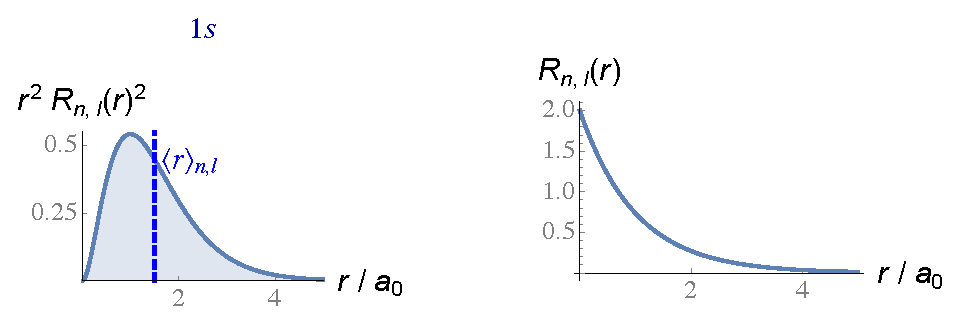
\includegraphics[scale=0.65]{Imagenes/Plot_Funcion_Radial_10.eps}
\end{figure}
\end{frame}
\begin{frame}
\frametitle{La función $R_{20}$}
\begin{align*}
R_{20} = \dfrac{1}{\sqrt{2}} \, a^{-3/2} \, \left( 1 - \dfrac{1}{2} \, \dfrac{r}{a} \right)\exp(-\dfrac{r}{2a})
\end{align*}
\pause
\vspace*{-0.5cm}
\begin{figure}
   \centering
   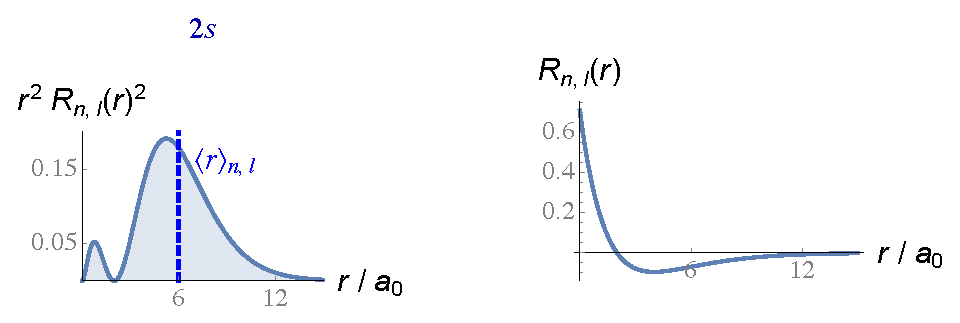
\includegraphics[scale=0.67]{Imagenes/Plot_Funcion_Radial_20.eps}
\end{figure}
\end{frame}
\begin{frame}
\frametitle{La función $R_{21}$}
\begin{align*}
R_{21} = \dfrac{1}{\sqrt{24}} \, a^{-3/2} \, \dfrac{r}{a} \, \exp(-\dfrac{r}{2a})
\end{align*}
\pause
\vspace*{-0.5cm}
\begin{figure}
   \centering
   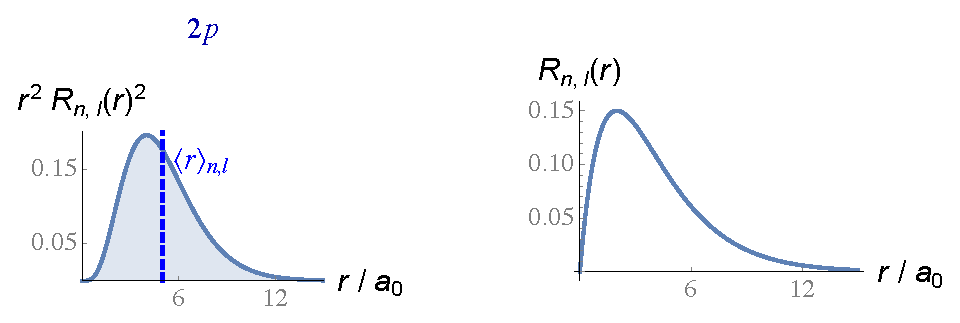
\includegraphics[scale=0.67]{Imagenes/Plot_Funcion_Radial_21.eps}
\end{figure}
\end{frame}
\begin{frame}
\frametitle{La función $R_{30}$}
\begin{align*}
R_{30} = \dfrac{2}{\sqrt{27}} \, a^{-3/2} \, \left[ 1 {-} \dfrac{2}{3} \, \dfrac{r}{a} {+} \dfrac{2}{27} \, \left( \dfrac{r}{a} \right)^{2} \right] \, \exp(-\dfrac{r}{3a})
\end{align*}
\pause
\vspace*{-0.5cm}
\begin{figure}
   \centering
   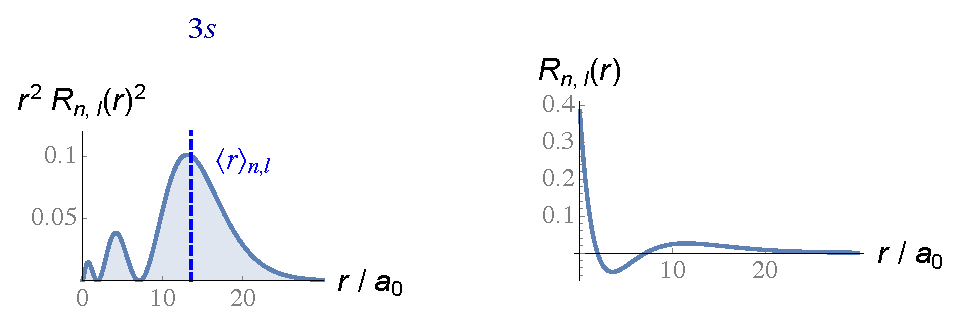
\includegraphics[scale=0.67]{Imagenes/Plot_Funcion_Radial_30.eps}
\end{figure}
\end{frame}
\begin{frame}
   \frametitle{La función $R_{31}$}
\begin{figure}
   \centering
   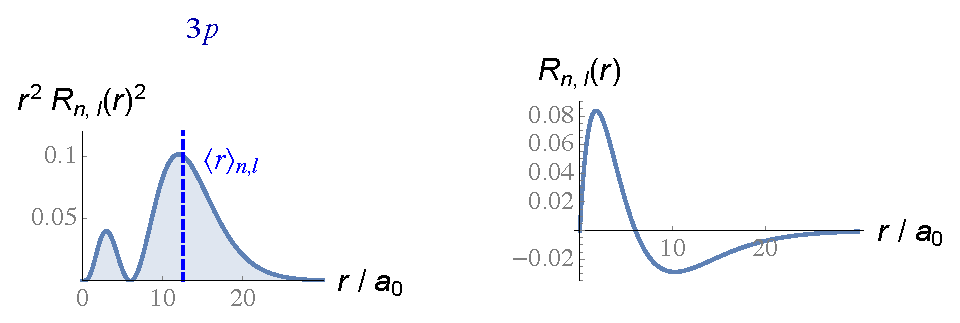
\includegraphics[scale=0.67]{Imagenes/Plot_Funcion_Radial_31.eps}
\end{figure}
\end{frame}
\begin{frame}
\frametitle{La función $R_{32}$}
\begin{figure}
   \centering
   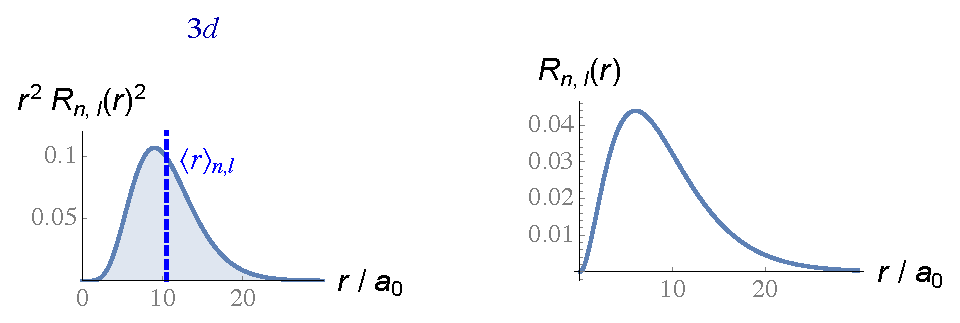
\includegraphics[scale=0.67]{Imagenes/Plot_Funcion_Radial_32.eps}
\end{figure}
\end{frame}
\begin{frame}
\frametitle{La función $R_{40}$}
\begin{figure}
   \centering
   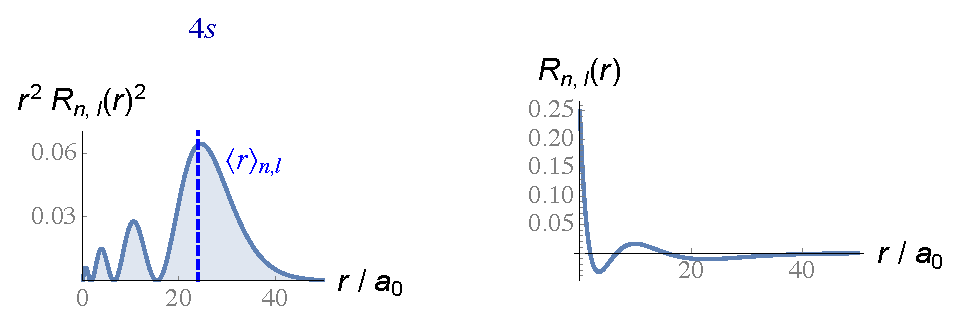
\includegraphics[scale=0.67]{Imagenes/Plot_Funcion_Radial_40.eps}
\end{figure}
\end{frame}
\begin{frame}
\frametitle{La función $R_{41}$}
\begin{figure}
   \centering
   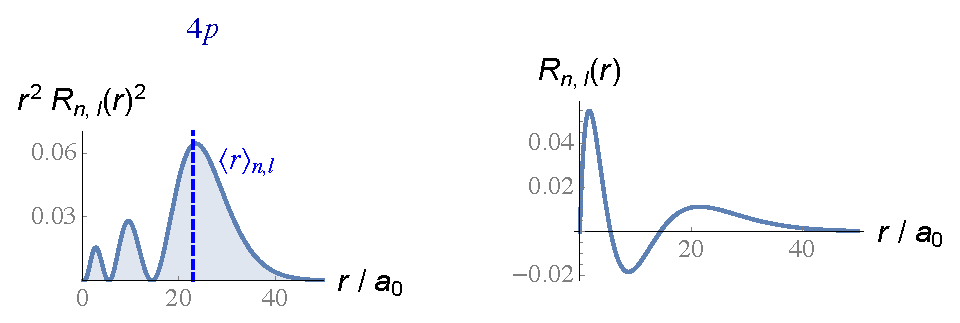
\includegraphics[scale=0.67]{Imagenes/Plot_Funcion_Radial_41.eps}
\end{figure}
\end{frame}
\begin{frame}
\frametitle{La función $R_{42}$}
\begin{figure}
   \centering
   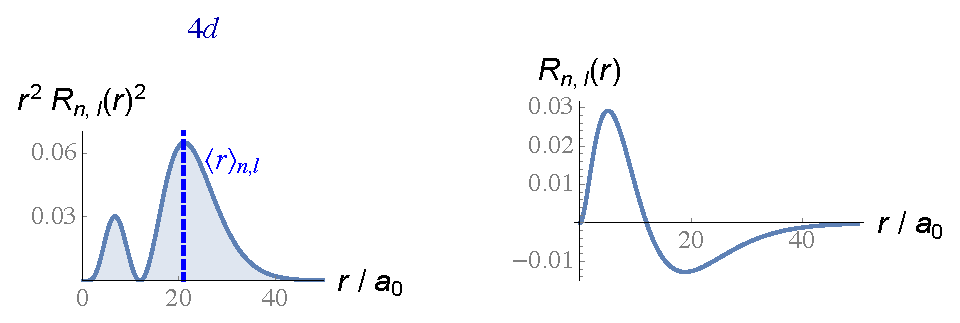
\includegraphics[scale=0.67]{Imagenes/Plot_Funcion_Radial_42.eps}
\end{figure}
\end{frame}
\begin{frame}
\frametitle{La función $R_{43}$}
\begin{figure}
   \centering
   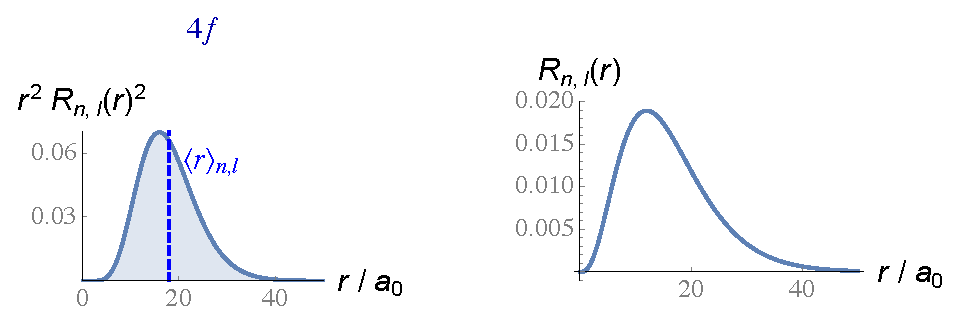
\includegraphics[scale=0.67]{Imagenes/Plot_Funcion_Radial_43.eps}
\end{figure}
\end{frame}
    
\end{document}